\section{Decay Angles}

\begin{frame}{Decay Angles}
\begin{itemize}

    \Item TGenPhaseSpace simulates decays in the rest frame of the decay parent.
        In this frame, all decay pairs decay in opposite directions, so the
        decay angle is 180$\degree$.
    
    \Item I'm interested in what this angle looks like in the \emph{lab frame}.
        In other words, in the frame relativistically boosted by the Lorentz
        vector of the decay parent. These are typically moving with $v \sim c$,
        so where in the rest frame two particles decayed 180$\degree$ apart, in
        the lab frame the angle is very small.
    
    \Item The distribution of this angle allows us to distinguish the important
        decays that we are looking for from the background.

\end{itemize}
\end{frame}

\begin{frame}{Decay Angles}

\begin{figure}
    \begin{center}
    \def\svgwidth{\columnwidth}
    \input{graphics/DecayAngle.pdf_tex}
    \end{center}
\end{figure}
\end{frame}

\subsection{$\psi(3770) \rightarrow D^0 \xbar{D^0}$}

\begin{frame}{$\psi(3770) \rightarrow D^0 \xbar{D^0}$}
\begin{itemize}

    \Item Before the decay angle in the lab frame can be calculated, first you
        need the Lorentz vector of the parent $\psi(3770)$.
    
    \Item To this end, momentum component distributions were obtained from a
        LHCb Monte Carlo simulation.
    
    \Item These momentum component distributions were fitted to mathematical
        functions.
    
    \Item The MC simulation of the $\psi(3770) \rightarrow D^0 \xbar{D^0}$ decay
        was then repeated a large number of times and each time the products'
        4-momenta were boosted by a random vector fitting the momentum
        distributions from the mathematical fit to the MC simulation.

\end{itemize}
\end{frame}

\begin{frame}{$\psi(3770) \rightarrow D^0 \xbar{D^0}$}

\begin{figure}
    \centering
    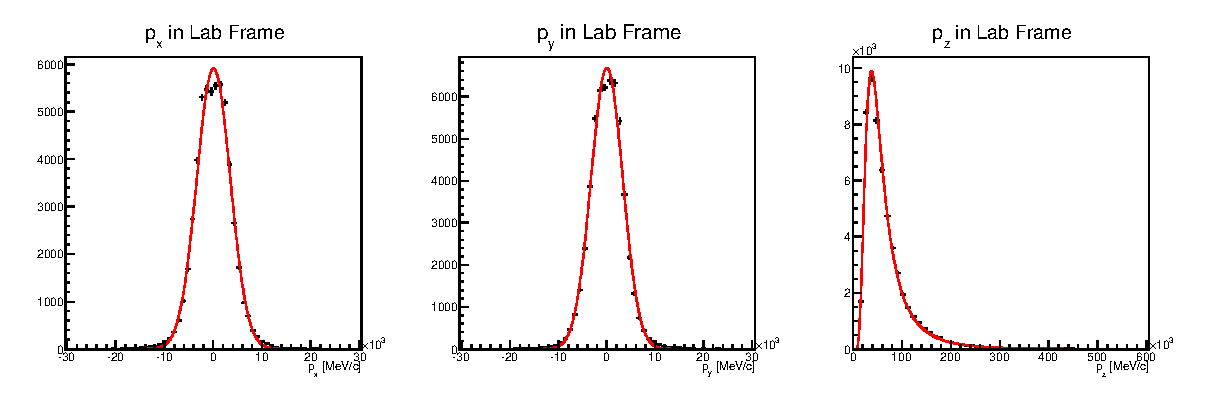
\includegraphics[width=1.1\linewidth]{graphs/PsiMomentumComponentFit.eps}
\end{figure}

Note that these are not perfect fits, but they are sufficiently accurate for our
purposes.
\end{frame}

\begin{frame}{$\psi(3770) \rightarrow D^0 \xbar{D^0}$}
\begin{itemize}

    \Item Need to confirm independence of $p_x$, $p_y$ and $p_z$ in order to use
        them independently for TGenPhaseSpace simulation.
    
    \Item Correlation factors between components calculated and tabulated:

    \begin{center}
  \begin{tabu}{| c |[1.25pt] c | c | c |}
    \hline
    & \LARGE $p_x$ & \LARGE $p_y$ & \LARGE $p_z$ \\
    \tabucline[1.25pt]{-}
    \LARGE $p_x$ & 1 &  0.00640212 & 0.0150375 \\
    \hline
    \LARGE $p_y$ & 0.00640212 & 1 & 0.0167604 \\
    \hline
    \LARGE $p_z$ & 0.0150375 & 0.0167604 & 1 \\
    \hline
  \end{tabu}
  \captionof{table}{The correlation factors between each momentum component. Note that
      these are all extremely low, thus the components can be considered
      independent of one another.}
  \label{tab:psi-correlation-factors}
\end{center}


    \Item Following plots visualise this independence:

\end{itemize}
\end{frame}

\begin{frame}{$\psi(3770) \rightarrow D^0 \xbar{D^0}$}

\begin{figure}
    \centering
    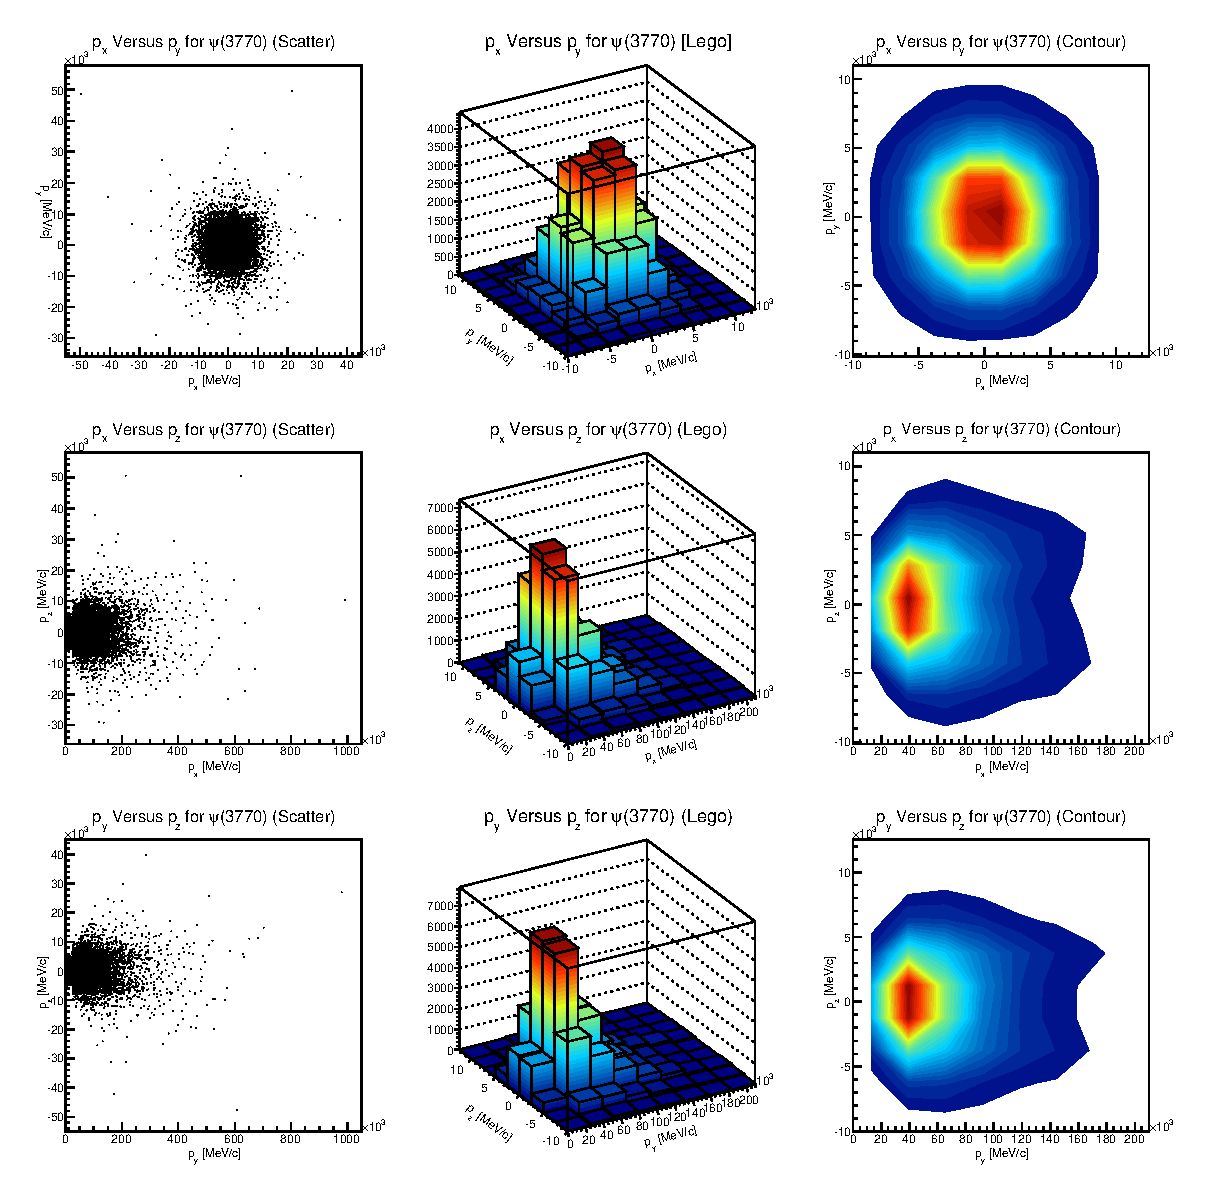
\includegraphics[scale=0.35]{graphs/PsiMomentumComponentCorrelation.eps}
\end{figure}
\end{frame}

\begin{frame}{$\psi(3770) \rightarrow D^0 \xbar{D^0}$}

Final plot of decay angle between $D^0$ and $\xbar{D^0}$ in lab frame:

\begin{figure}
    \begin{center}
    \includegraphics[width=\linewidth]{graphs/PsiBoostedAngle.eps}
    \end{center}
\end{figure}

Note that all decays are below $\simeq 5\degree$.
\end{frame}

\begin{frame}{$\psi(3770) \rightarrow D^0 \xbar{D^0}$}
\begin{itemize}

    \Item Importance of this graph is that the decay angle is highly peaked
        around $\sim 0.5\degree$
    
    \Item This makes it very useful for distinguishing this interesting decay
        channel from the uninteresting background, which should not be peaked
        but more evenly angularly distributed (although it may have some angular
        dependence).

\end{itemize}
\end{frame}

\subsection{$B \rightarrow (\psi(3770) \rightarrow D^0 \xbar{D^0})K$}

\begin{frame}{$B \rightarrow (\psi(3770) \rightarrow D^0 \xbar{D^0})K$}
\begin{itemize}

    \Item The same was done of the $B$ meson, using LHCb MC momentum data for $B
        \rightarrow D~Bach$ decay. (The $Bach$ is either a kaon or a pion.)
    
    \Item However, no $B$ momentum data present, so used conservation of
        momentum to deduce $B$ momentum components from the sum of the product
        $D$ and $Bach$ mesons, using $P_{B,i} = P_{D,i} + P_{Bach,i}$ for $i \in
        \{x,y,z\}$. 
    
    \Item Correlation factor matrix:

    \begin{center}
  \begin{tabu}{| c |[1.25pt] c | c | c |}
    \hline
    & \LARGE $p_x$ & \LARGE $p_y$ & \LARGE $p_z$ \\
    \tabucline[1.25pt]{-}
    \LARGE $p_x$ & 1 &  0.0165178 & -0.00486466 \\
    \hline
    \LARGE $p_y$ & 0.0165178 & 1 & 0.017408 \\
    \hline
    \LARGE $p_z$ & -0.00486466 & 0.017408 & 1 \\
    \hline
  \end{tabu}
  \captionof{table}{The correlation factors of the momentum components of the
      $B$ meson, obtained from LHCb $B \rightarrow D~Bach$ MC data.}
  \label{tab:b-correlation-factors}
\end{center}


\end{itemize}
\end{frame}

\begin{frame}{$B \rightarrow (\psi(3770) \rightarrow D^0 \xbar{D^0})K$}

\begin{figure}
    \begin{center}
    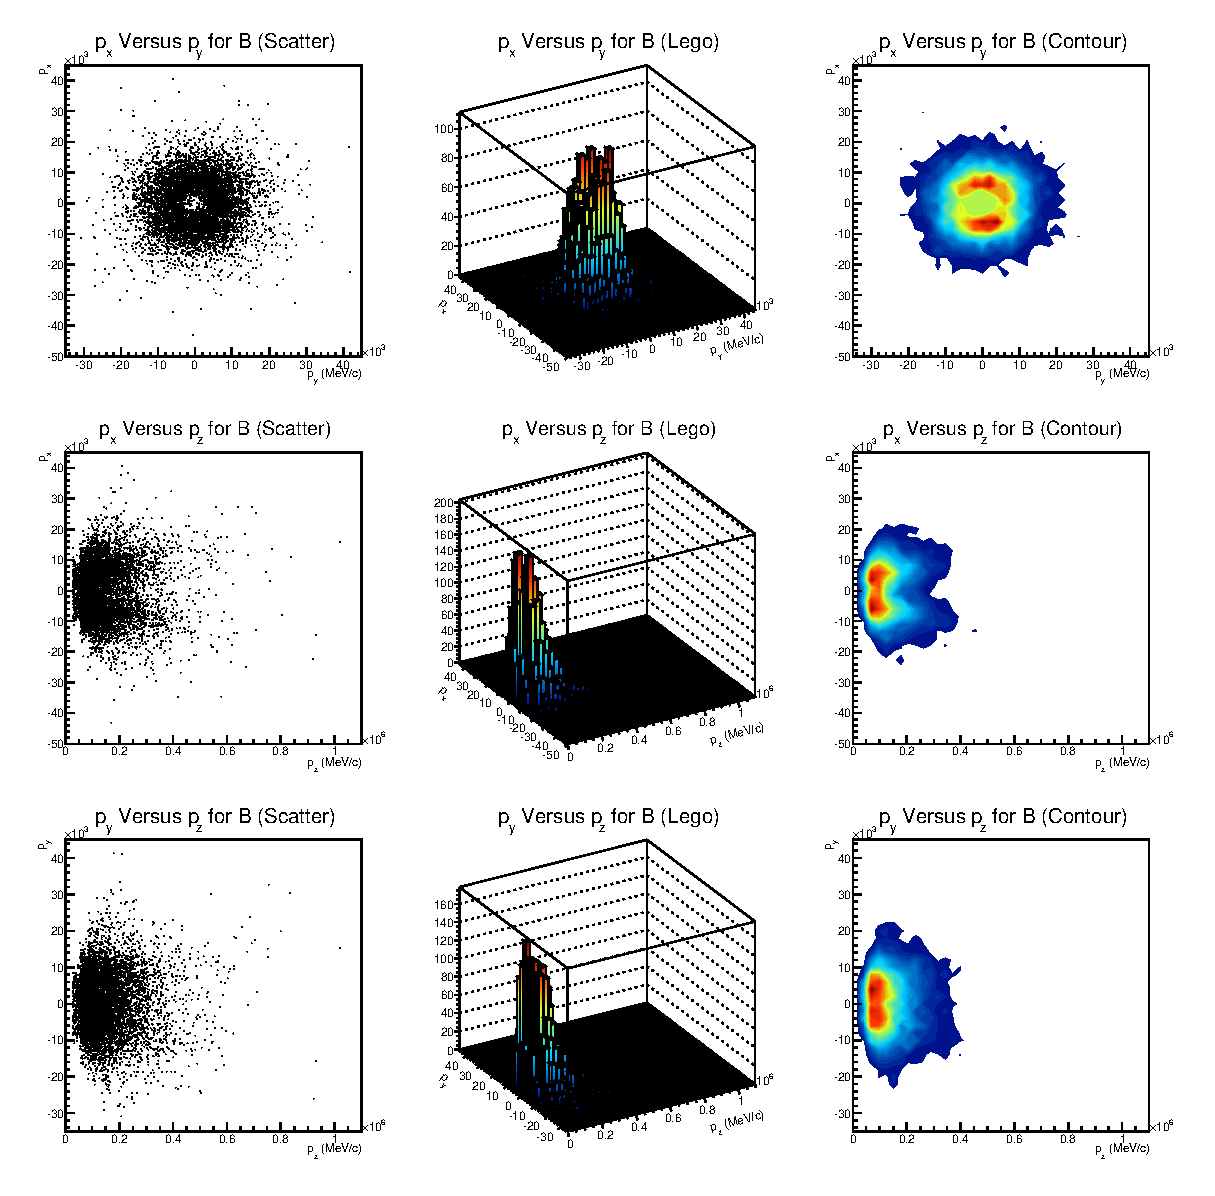
\includegraphics[scale=0.35]{graphs/BMomentumComponentCorrelation.eps}
    \end{center}
\end{figure}
\end{frame}

\begin{frame}{$B \rightarrow (\psi(3770) \rightarrow D^0 \xbar{D^0})K$}

\begin{figure}
    \begin{center}
    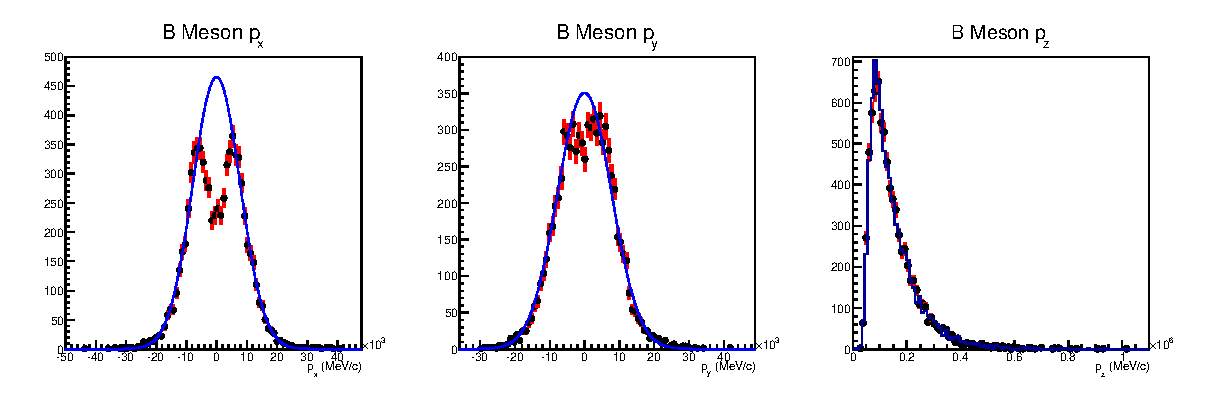
\includegraphics[width=1.1\linewidth]{graphs/BMomentumComponentFit.eps}
    \end{center}
\end{figure}
\end{frame}

\begin{frame}{$B \rightarrow (\psi(3770) \rightarrow D^0 \xbar{D^0})K$}
\begin{center}
\textbf{Final decay angle graphs:}
\end{center}

In rest frame of parent $B$:
\begin{figure}
    \begin{center}
    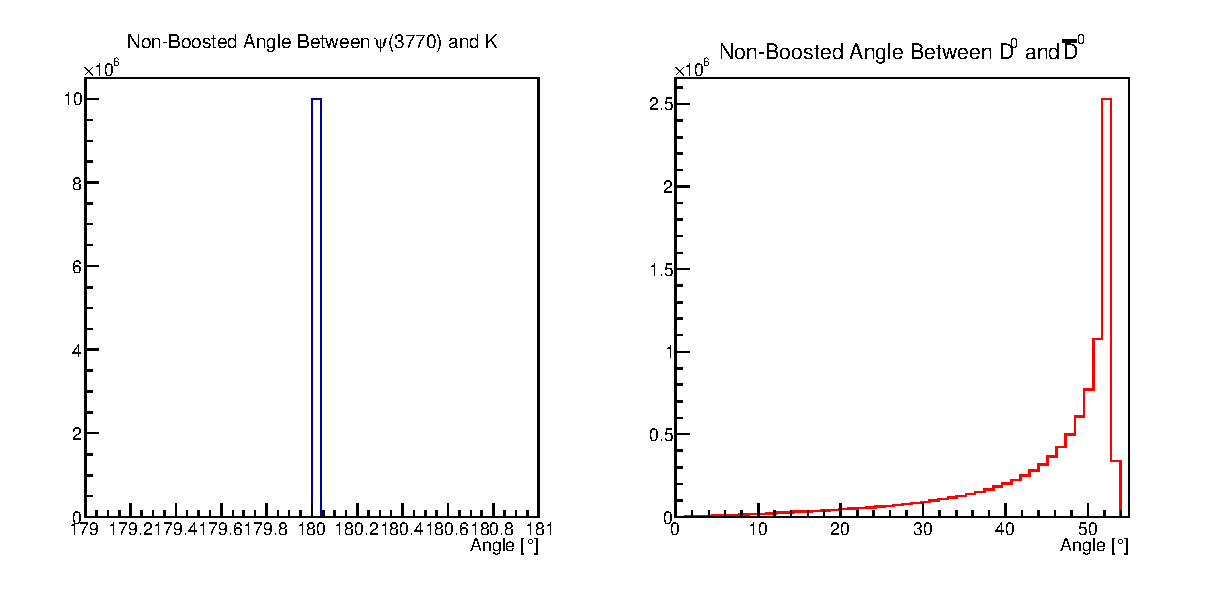
\includegraphics[width=\linewidth]{graphs/BMomentumNonBoostAngle.eps}
    \end{center}
\end{figure}
\end{frame}

\begin{frame}{$B \rightarrow (\psi(3770) \rightarrow D^0 \xbar{D^0})K$}
In lab frame:

\begin{figure}
    \begin{center}
    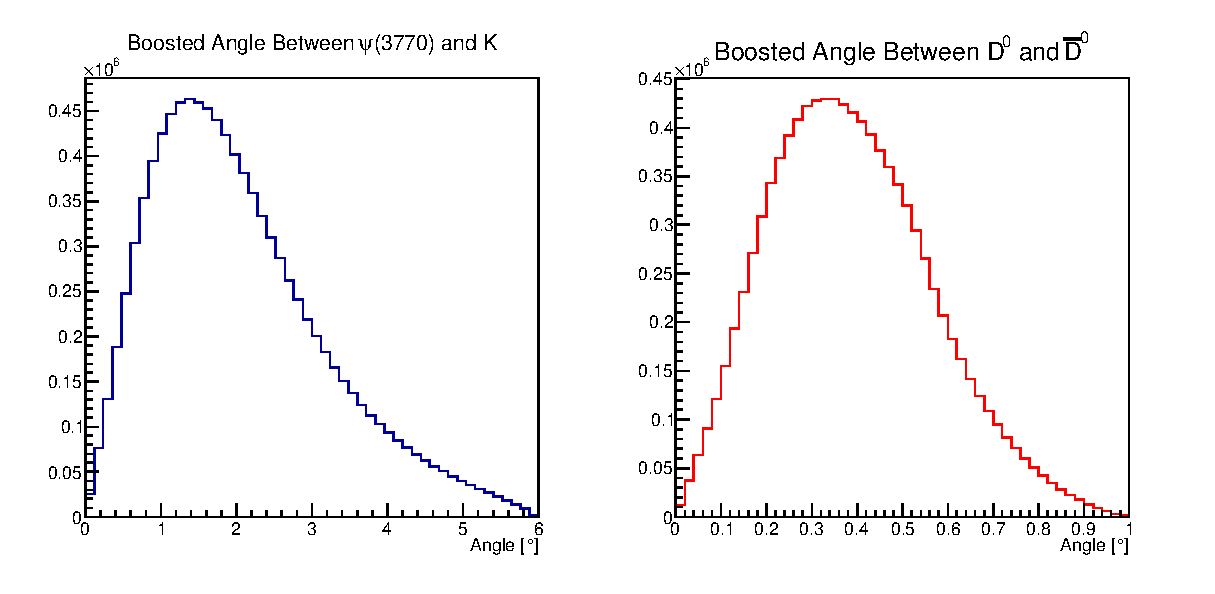
\includegraphics[width=\linewidth]{graphs/BMomentumBoostAngle.eps}
    \end{center}
\end{figure}
\end{frame}

\begin{frame}{$B \rightarrow (\psi(3770) \rightarrow D^0 \xbar{D^0})K$}
\begin{itemize}

    \Item Once again, we find that the decay angle is sharply peaked around
        $\simeq 1.5\degree$ for the $\psi(3770)-K$ angle and $\simeq 0.4\degree$
        for the $D^0-\xbar{D^0}$ angle.
    
    \Item This is good, because it means that the decay angle can accurately be
        used to distinguish this interesting decay from all the uninteresting
        background decays going on.
    
    \Item This allows us to isolate more $\psi(3770)$ decays for symmetry
        violation studies.

\end{itemize}
\end{frame}
